% -*- mode: latex; tex-main-file: "abstract.tex" -*-
\preparagraphspacing{}
\section*{Change Descriptors}
\label{sec:chdescs}

The ability to revert and re-apply change descriptors is inspired by the soft
updates system in BSD's FFS~\cite{ganger00soft}, but it is generalized so that
it is not specific to any particular filesystem. A simplified version of the
change descriptor structure is shown in Figure~\ref{fig:chdesc}.

\begin{figure}
{\footnotesize
\begin{verbatim}
struct chdesc {
    BD_t *device;
    bdesc_t *block;
    enum {BIT, BYTE, NOOP} type;
    union {
        struct {
            uint16_t offset;
            uint32_t xor;
        } bit;
        struct {
            uint16_t offset, length;
            uint8_t *data;
        } byte;
    };
    struct chdesc *dependencies[];
};
\end{verbatim}
}
\vspace{-14pt}
\caption{\label{fig:chdesc} Change descriptor structure.}
\end{figure}

When a KudOS module first generates change descriptors to write to the disk, it
specifies write ordering requirements similar to those of soft updates. For
example, Figure~\ref{fig:softupdates} depicts change descriptors that allocate
and add a new block to an inode.
%
The module passes these change descriptors to another module in the direction of
the disk, which can inspect, delay, and even modify them before passing them on.
%
For instance, the write-back cache module holds onto blocks and their change
descriptors instead of passing them on immediately.
%
When a block must be evicted, it makes sure to send change descriptors toward
the disk in an order consistent with the change descriptor dependency
information.

\begin{figure}[b]
  \centering
  \includegraphics[width=92pt]{fig/whatevs_3}%
  \caption{\label{fig:softupdates} Soft updates change descriptor graph,
  including the dependencies for adding a newly allocated block to an
  inode. Writing the new block pointer to an inode (Attach) depends on
  initializing the block (Clear) and updating the free block map (Alloc).
  Updating the size of the inode (Size) depends on writing the block
  pointer.}
\end{figure}

Soft updates, journalling, and many application-specific consistency models all
correspond to different change descriptor arrangements, so these features can be
added to the system as modules which appropriately connect or reconnect the
change descriptors. Figure~\ref{fig:softupdates} shows a set of change
descriptors which corresponds to adding a newly allocated block to an inode,
using soft updates consistency semantics. Figure~\ref{fig:journal} shows the
same change descriptors, but as a journal transaction. We have implemented
journalling as a single module (to which any filesystem module can be attached)
that transforms input change descriptor graphs like that in
Figure~\ref{fig:softupdates} to output graphs like Figure~\ref{fig:journal}.

\begin{figure}
  \centering
  \includegraphics[width=\hsize]{fig/whatevs_2}%
  \caption{\label{fig:journal} Journal change descriptor graph for the
  change in Figure~\ref{fig:softupdates}.  The original four change
  descriptors depend on a journal commit record, which depends on blocks
  being written to the journal.  Once the actual changes are committed, the
  journal record is marked as completed.  Empty circles are ``NOOP'' change
  descriptors with no associated block data.  }
\end{figure}

Even metadata-only journalling is possible with this design, though our journal
module does not yet have this feature. Other block device layering systems, like
GEOM~\cite{geom} or JBD in Linux, would or do need special hooks into filesystem
code in order to get the necessary hints (i.e. what is metadata and what is not)
to do metadata-only journalling. Change descriptors (and the LFS interface
division described in the next section) allow us to do this automatically.

Another advantage of passing change descriptors around like this is that
dependency information can be maintained even across boundaries that might
otherwise lose that information, like loopback devices or RAID. With KudOS,
consistency requirements of filesystems mounted using loopback devices can
easily be respected even though the filesystem containing the loopback image
file may not itself use any consistency features. Similarly, when using RAID,
the change descriptors can be modified so that as they part ways in the RAID
module toward different disks, their write-ordering requirements are still
maintained and ultimately satisfied.

%\begin{figure}
%  \centering
%  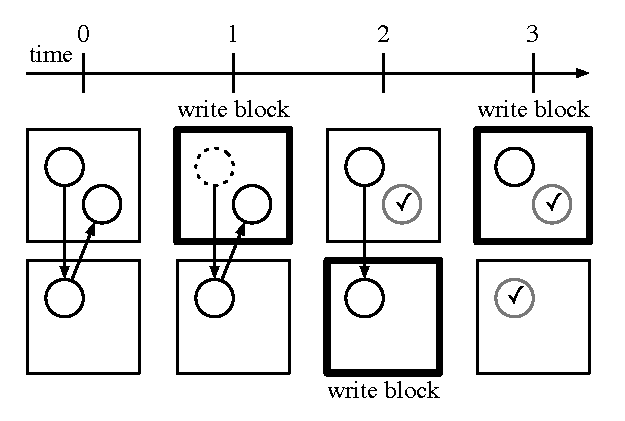
\includegraphics[width=200pt]{rollback_sequence}
%  \caption{\label{fig:rollback} Rolling back change descriptors. Although no
%  cycles are allowed in change descriptor graphs, cycles can exist at the block
%  level which require some change descriptors to be rolled back in order to
%  write the blocks. Here the squares are disk blocks, and dotted circles are
%  rolled back change descriptors. Check marks indicate committed change
%  descriptors.
%}
%\end{figure}
